\begin{figure}[h]
  \centering
  \tikzstyle{vertex}=[]
  \tikzstyle{arrow}=[thick, -latex]
  \tikzstyle{hidden}=[gray!50]

  \begin{subfigure}[b]{1.4in}
    \centering
    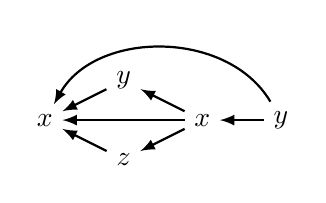
\begin{tikzpicture}
      \node[vertex] (x1) at (0, 0) {$x$};
      \node[vertex] (y1) at (1, 0.5) {$y$};
      \node[vertex] (y2) at (1, -0.5) {$z$};
      \node[vertex] (x2) at (2, 0) {$x$};
      \node[vertex] (z) at (3, 0) {$y$};

      \draw[arrow] (y1) to (x1);
      \draw[arrow] (y2) to (x1);
      \draw[arrow] (x2) to (y1);
      \draw[arrow] (x2) to (y2);
      \draw[arrow] (x2) to (x1);
      \draw[arrow, bend right=60] (z) to (x1);
      \draw[arrow] (z) to (x2);
    \end{tikzpicture}
    \caption{A conflict graph $C$}\figlabel{ExampleConflictGraph}
  \end{subfigure}%
  \hspace{0.5in}
  %
  \begin{subfigure}[b]{1.4in}
    \centering
    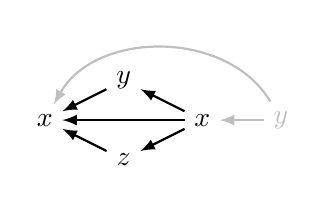
\begin{tikzpicture}
      \node[vertex] (x1) at (0, 0) {$x$};
      \node[vertex] (y1) at (1, 0.5) {$y$};
      \node[vertex] (y2) at (1, -0.5) {$z$};
      \node[vertex] (x2) at (2, 0) {$x$};
      \node[vertex, hidden] (z) at (3, 0) {$y$};

      \draw[arrow] (y1) to (x1);
      \draw[arrow] (y2) to (x1);
      \draw[arrow] (x2) to (y1);
      \draw[arrow] (x2) to (y2);
      \draw[arrow] (x2) to (x1);
      \draw[arrow, bend right=60, hidden] (z) to (x1);
      \draw[arrow, hidden] (z) to (x2);
    \end{tikzpicture}
    \caption{A suffix of $C$}\figlabel{ExampleSuffix}
  \end{subfigure}%
  \hspace{0.5in}
  %
  \begin{subfigure}[b]{1.4in}
    \centering
    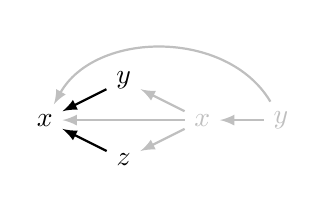
\begin{tikzpicture}
      \node[vertex] (x1) at (0, 0) {$x$};
      \node[vertex] (y1) at (1, 0.5) {$y$};
      \node[vertex] (y2) at (1, -0.5) {$z$};
      \node[vertex, hidden] (x2) at (2, 0) {$x$};
      \node[vertex, hidden] (z) at (3, 0) {$y$};

      \draw[arrow] (y1) to (x1);
      \draw[arrow] (y2) to (x1);
      \draw[arrow, hidden] (x2) to (y1);
      \draw[arrow, hidden] (x2) to (y2);
      \draw[arrow, hidden] (x2) to (x1);
      \draw[arrow, bend right=60, hidden] (z) to (x1);
      \draw[arrow, hidden] (z) to (x2);
    \end{tikzpicture}
    \caption{Another suffix of $C$}\figlabel{ExampleSuffix2}
  \end{subfigure}

  \caption{}
\end{figure}
